\documentclass[11pt,oneside]{scrbook}
\usepackage[a4paper,margin=2.4cm,marginparwidth=1.8cm,marginparsep=0.4cm]{geometry}
\usepackage{../common/rlstudy}

\title{{\color{rlblue}\textbf{Week 22} \\ \Huge Constrained MDPs, Lagrangian Methods, CPO, FOCOPS, P3O}}
\author{STUDY-RL --- a self-paced Deep RL curriculum}
\date{\today}

\begin{document}
\maketitle
\tableofcontents
\newpage

% =====================================================================
\chapter*{Learning objectives}
\addcontentsline{toc}{chapter}{Learning objectives}


% Teaching companion: a small example before the full lecture.
\noindent\textbf{Study companion.} Read \texttt{teaching\_guide.md} in this
folder for step-by-step examples, an analogy with its limits, and self-checks.
Then use \texttt{workbook.ipynb} to implement and vary the calculations.
\par\medskip

\begin{keyidea}
By the end of this lecture you will be able to:
\begin{enumerate}[leftmargin=*]
  \item State Altman's Constrained MDP (CMDP) formulation as both a constrained
        optimisation in policy space and as a linear program in
        occupancy-measure space.
  \item Derive the Lagrangian relaxation step-by-step, identify the saddle-point
        and write the primal-dual algorithm.
  \item Implement PPO-Lagrangian end-to-end: dual advantage, projected
        multiplier update by projected descent on $L$, gradient-clipping, and the variance-control tricks
        (advantage normalisation, cost-scale normalisation).
  \item Derive the CPO trust-region update from first principles, including
        the closed-form solution of the constrained quadratic program.
  \item State and apply the FOCOPS closed-form non-parametric optimum and the
        P3O exact-penalty argument.
  \item Define a coherent risk measure, derive Conditional Value-at-Risk,
        and read off CVaR from a distributional critic.
  \item Diagnose the two canonical failure modes of Lagrangian RL (multiplier
        oscillation, cost-scale mismatch) and explain why PID-Lagrangian
        damps them.
\end{enumerate}
\end{keyidea}

% =====================================================================
\chapter{Motivation \& intuition}

\section{The hard problem nobody told you about}

Up to week 21 we have been maximising expected return $J_r(\pi)
= \E_\pi [\sum_t \gamma^t r_t]$. In practice this is rarely what we actually
want.\footnote{In recruiting, a ``return'' might be ``successful hires'' and a
``cost'' might be ``rate of demographic-parity violation''. Maximising one with
zero regard for the other is an excellent way to build a discrimination-as-a-service
product.}
The deployer almost always also cares about a side-quantity that must not
blow up: an energy budget, a collision count, an unfairness metric, a maximum
exposure to a particular candidate group, a clinical safety event rate.

In the unconstrained formulation those concerns get baked into the reward
through a hand-tuned scalar: $r_t - \beta\, c_t$. This is brittle. The chosen
$\beta$ is almost always either too soft (constraint violated) or too harsh
(reward collapses). Worse, the trade-off interpretation of $\beta$ is
\emph{not} preserved during training --- the agent has no view of the global
constraint, only of the local linear combination.

The Constrained MDP framework promotes that scalar to a first-class variable
$\lambda \geq 0$ that the algorithm \emph{learns}, by formal duality. The
result is a primal-dual algorithm that\footnote{This is exactly the same
trick that turns Support-Vector-Machine training into the dual problem you
saw in your ML course: a constrained quadratic program with KKT conditions,
solved by alternating primal--dual updates.}
solves \emph{the right problem} --- maximise reward subject to constraint.

\section{Three mental models}

\begin{intuition}\textbf{The thermostat analogy.}
$\lambda$ is the price of cost. When the agent is overspending the budget,
prices rise and the policy starts avoiding cost; when it is underspending,
prices fall and the policy can afford to chase reward more aggressively. The
equilibrium price is the marginal value of one extra unit of budget.
\end{intuition}

\begin{intuition}\textbf{The market analogy.}
Each (state, action) pair has two coupons: $r(s,a)$ and $c(s,a)$. The dual
variable $\lambda$ is the exchange rate between them. The optimal policy
trades reward for cost at exactly that exchange rate; at any other rate, the
budget is either wasted (slack constraint) or violated.
\end{intuition}

\begin{intuition}\textbf{The KKT analogy.}
At the saddle point of the Lagrangian we have stationarity (policy gradient
zero), primal feasibility ($J_c \leq d$), dual feasibility ($\lambda \geq 0$),
and complementary slackness ($\lambda (J_c - d) = 0$). Same KKT conditions you
saw in convex analysis --- but evaluated through Monte-Carlo estimates on
policy-induced trajectory distributions.
\end{intuition}

% =====================================================================
\chapter{Mathematical formulation}

\section{Altman's CMDP}

\begin{definition}[Constrained MDP]\label{def:cmdp}
A \emph{constrained Markov Decision Process} is a tuple
$\mathcal{M} = (\States, \Actions, P, r, c, \gamma, d)$ where
$(\States, \Actions, P, r, \gamma)$ is a standard discounted MDP and
$c : \States \times \Actions \to \Real_{\geq 0}$ is a \emph{cost function}
with budget $d \geq 0$. The objective is
\[
   \max_\pi\;\; J_r(\pi) \;\defeq\; \E_\pi\!\left[\sum_{t \geq 0} \gamma^t r(s_t, a_t)\right]
   \quad \text{subject to} \quad
   J_c(\pi) \;\defeq\; \E_\pi\!\left[\sum_{t \geq 0} \gamma^t c(s_t, a_t)\right] \;\leq\; d.
\]
\end{definition}

In full generality there can be several cost channels with separate budgets;
we keep one for clarity.

\paragraph{The LP view.}
For a finite CMDP, the \emph{discounted state-action occupancy measure}
\[
  \mu^\pi(s,a) \;=\; (1-\gamma) \sum_{t \geq 0} \gamma^t \Prb_\pi(s_t = s, a_t = a)
\]
satisfies $\sum_{s,a} \mu^\pi(s,a) = 1$ and the Bellman-flow constraint
\[
  \sum_a \mu(s,a) \;=\; (1-\gamma)\rho_0(s) + \gamma \sum_{s',a'} P(s\mid s',a')\, \mu(s',a').
\]
The CMDP becomes a linear program over the polytope of valid occupancies:
\[
  \max_\mu\; \tfrac{1}{1-\gamma}\!\sum_{s,a} \mu(s,a)\, r(s,a)
  \;\;\text{s.t.}\;\; \tfrac{1}{1-\gamma}\!\sum_{s,a} \mu(s,a)\, c(s,a) \leq d,
  \;\; \text{Bellman flow}.
\]
Because there are $m$ scalar constraints, an optimal vertex of this polytope
needs at most $m$ randomisations beyond the basic deterministic feasible set
--- this is \textsc{Altman, 1999}'s classical structural theorem. In practice
it means the \emph{optimal policy in a CMDP can be stochastic} even when the
unconstrained optimum was deterministic --- a fact you must internalise before
you start debugging your safety algorithms.

\begin{pitfall}
\textbf{Determinism bias.} Many practitioners default to deterministic policies
because TD3/DDPG/SAC-tuned habits push that way. In a CMDP a constraint
\emph{may require randomisation at the optimal tight solution}.
A deterministic policy can be feasible or even optimal, but restricting
to deterministic policies can lose value or feasibility in some CMDPs.
\end{pitfall}

\section{The Lagrangian and its saddle-point}

Form the (one-constraint) Lagrangian
\begin{equation}\label{eq:lagrangian}
   L(\pi, \lambda) \;=\; J_r(\pi) - \lambda\, \bigl( J_c(\pi) - d \bigr), \qquad \lambda \geq 0.
\end{equation}

\begin{theorem}[Strong duality for finite CMDPs]\label{thm:strong-dual}
If the CMDP from \cref{def:cmdp} is feasible (i.e., there exists $\pi_0$
with $J_c(\pi_0) < d$, Slater's condition), then strong duality holds:
\[
   \max_\pi \min_{\lambda \geq 0} L(\pi, \lambda) \;=\; \min_{\lambda \geq 0} \max_\pi L(\pi, \lambda).
\]
A primal-dual optimal pair $(\pi^\star, \lambda^\star)$ exists and the KKT
conditions are
\[
\begin{aligned}
   \text{primal feas.}\quad & J_c(\pi^\star) \leq d, \\
   \text{dual feas.}\quad & \lambda^\star \geq 0, \\
   \text{compl. slack.}\quad & \lambda^\star (J_c(\pi^\star) - d) = 0, \\
   \text{stationarity}\quad & \pi^\star \in \argmax_\pi \; J_r(\pi) - \lambda^\star J_c(\pi).
\end{aligned}
\]
\end{theorem}

\begin{proof}[Proof sketch]
Re-write the CMDP as the LP above. The feasible polytope is bounded by Bellman
flow + simplex constraints + the linear cost constraint. The dual LP
has variables $\lambda \geq 0$ (for the cost constraint) and free variables
for the Bellman-flow constraints. Slater $\Rightarrow$ the primal LP is strictly
feasible $\Rightarrow$ strong duality for LP (no gap). KKT is the LP
optimality criterion. Translating dual variables back to policies: the
inner $\max_\pi$ at fixed $\lambda$ is an unconstrained MDP with reward
$r - \lambda c$, hence has a deterministic optimum --- and a randomisation
between two such MDPs (corresponding to $\lambda \pm \epsilon$) realises the
constrained optimum.
\end{proof}

\begin{remark}
For deep RL, the inner $\max_\pi$ at fixed $\lambda$ is approximate (truncated
gradient ascent on the surrogate). We do not get exact KKT in finite time;
convergence requires additional assumptions on optimisation, estimation,
feasibility, and timescales. A Robbins--Monro multiplier step-size schedule
alone does not guarantee a saddle point for a neural policy.
\end{remark}

\section{Deriving the primal-dual update}

Suppose $\pi_\theta$ is parametrised by $\theta$. We want to ascend $L$ in
$\theta$ and descend $L$ in $\lambda$:
\[
   \theta_{k+1} = \theta_k + \eta_\theta\, \nabla_\theta L(\pi_{\theta_k}, \lambda_k)
   = \theta_k + \eta_\theta\, \bigl( \nabla_\theta J_r(\pi_{\theta_k}) - \lambda_k\, \nabla_\theta J_c(\pi_{\theta_k}) \bigr).
\]
Both gradients are policy-gradient quantities:
\[
   \nabla_\theta J_r(\pi_\theta) = \E_{\pi_\theta}\!\left[ \sum_t \nabla_\theta \log \pi_\theta(a_t|s_t)\, A^{\pi_\theta}_r(s_t, a_t) \right],
\]
and analogously for cost. The combined gradient uses the
\emph{augmented advantage}
\begin{equation}\label{eq:aug-adv}
   A^{\text{tot}}(s,a) \;=\; A_r(s,a) - \lambda\, A_c(s,a),
\end{equation}
which is the cleanest object to remember from this lecture.

For the multiplier we use projected gradient descent on $L$ at fixed $\pi$. Since $\partial L/\partial\lambda=-(J_c-d)$, descent increases $\lambda$ when cost exceeds the budget:
\begin{equation}\label{eq:dual-update}
  \lambda_{k+1} \;=\; \bigl[\, \lambda_k + \eta_\lambda\, \bigl( \hat{J}_c(\pi_{\theta_k}) - d \bigr) \,\bigr]_+ .
\end{equation}
$\hat{J}_c$ is the Monte-Carlo estimate from the current rollout.

\paragraph{Why we don't simply use $r - \beta c$.}
A fixed $\beta$ is \emph{exactly} the Lagrangian \emph{at the optimum} $\beta
= \lambda^\star$. Of course we do not know $\lambda^\star$ a priori. The
primal-dual loop computes it for us.

\section{The CPO trust-region update}

\textsc{Achiam et al.\ 2017} (arXiv:1705.10528) gave the first deep-RL
algorithm with a per-iteration constraint-satisfaction guarantee. The key
inequality, derived from the standard performance-difference lemma (Kakade \&
Langford 2002):
\begin{equation}\label{eq:cpo-bound}
   J_c(\pi') - J_c(\pi) \;\leq\;
   \tfrac{1}{1-\gamma}\; \E_{s \sim d^\pi, a \sim \pi'}\!\bigl[ A_c^\pi(s,a) \bigr]
   \;+\; \tfrac{\sqrt{2}\, \gamma\, \epsilon_c^\pi}{(1-\gamma)^2}\, \sqrt{\bar D_\KL(\pi' \,\Vert\, \pi)},
\end{equation}
where $\epsilon_c^\pi \defeq \max_s |\E_{a\sim\pi'}[A_c^\pi(s,a)]|$ is a worst-case
cost-advantage scale. At each iteration CPO solves
\begin{equation}\label{eq:cpo-qp}
\begin{aligned}
  \theta_{k+1} = \argmax_\theta\;\; & g^\top (\theta - \theta_k) \\
  \text{s.t.}\;\; & b^\top (\theta - \theta_k) + c \;\leq\; 0, \\
  & \tfrac{1}{2} (\theta - \theta_k)^\top H (\theta - \theta_k) \;\leq\; \delta,
\end{aligned}
\end{equation}
where $g = \nabla_\theta J_r$, $b = \nabla_\theta J_c$ (cost gradient
evaluated under the current policy), $c = J_c(\pi_k) - d$ (current
constraint violation), $H$ the Fisher information of $\pi_\theta$ at
$\theta_k$, and $\delta$ is the trust-region radius.

\begin{theorem}[CPO closed-form update]\label{thm:cpo}
Define $q = g^\top H^{-1} g$, $r_{bg} = g^\top H^{-1} b$, $s_b = b^\top H^{-1} b$.
Assume $H$ is positive definite and $s_b>0$. The linearised constraint is feasible inside the trust region iff $c\le\sqrt{2\delta s_b}$. In the regular case with an active trust region, the optimal step is
\[
   \theta_{k+1} - \theta_k \;=\; \tfrac{1}{\lambda_\star}\, H^{-1} (g - \nu_\star b),
\]
where $\lambda_\star, \nu_\star$ solve the dual
\[
   \min_{\lambda \geq 0,\, \nu \geq 0} \;\; \tfrac{1}{2\lambda}\bigl(q - 2 \nu r_{bg} + \nu^2 s_b\bigr) - \nu c + \lambda \delta,\qquad\lambda>0.
\]
For an infeasible linearised constraint ($c > 0$ and the trust region cannot
satisfy it), CPO performs the \emph{recovery step}
$\theta_{k+1} = \theta_k - \sqrt{2\delta/s_b}\, H^{-1} b$, which is the
pure cost-reduction step inside the trust region.
\end{theorem}

\begin{proof}[Proof]
Form the Lagrangian
$\mathcal{L}(\theta, \lambda, \nu) = -g^\top(\theta-\theta_k) + \nu(b^\top(\theta-\theta_k) + c) + \lambda(\tfrac12 (\theta-\theta_k)^\top H (\theta-\theta_k) - \delta)$.
Stationarity in $\theta$ gives $(\theta-\theta_k) = H^{-1}(g - \nu b)/\lambda$.
Substituting back gives the concave dual of the negative-reward
minimisation. Negating that dual yields the displayed minimisation; this
changes both the $\nu c$ and $\lambda\delta$ signs. KKT classifies feasible vs.\ recovery regimes.
\end{proof}

CPO comes with a per-iteration bound:
$J_c(\pi_{k+1}) \leq d + (\text{trust-region slack})$, which decays as
$\sqrt{\delta}$.

\begin{pitfall}
\textbf{Fisher inversion.} $H^{-1} g$ in CPO is computed by conjugate gradients
on $Hv = g$, not by forming $H$ explicitly. Each CG iteration costs one
Hessian-vector product (forward + double backward through the log-policy).
For 24--32 GB single-GPU budgets, choose CG iterations \emph{at most} 10--20;
beyond that you pay more than the policy step itself.
\end{pitfall}

\section{FOCOPS --- first-order non-parametric optimum}

\textsc{Zhang, Vuong, Ross 2020} (arXiv:2002.06506). FOCOPS solves the same
problem as CPO but in non-parametric policy space (working point: at fixed
$\pi_k$, what is the optimal $\pi'$?), then projects.

Starting from the Lagrangian of the CPO QP \emph{in non-parametric form},
\[
   \max_{\pi'} \; \E_{s \sim d^{\pi_k}, a \sim \pi'}[A^{\pi_k}_r(s,a)]
   \;\;\text{s.t.}\;\; \E[A^{\pi_k}_c(s,a)] + c \leq 0,\;\; D_\KL(\pi' \Vert \pi_k) \leq \delta,
\]
and forming the Lagrangian $\mathcal{L}(\pi', \nu, \lambda)$, the KKT
stationarity in $\pi'(a|s)$ gives
\[
   \log \pi'(a|s) = \log \pi_k(a|s) + \tfrac{1}{\lambda}\bigl(A_r^{\pi_k}(s,a) - \nu A_c^{\pi_k}(s,a)\bigr) - 1 + \mu(s),
\]
where $\mu(s)$ is the multiplier on the row-normalisation $\sum_a \pi'(a|s) = 1$.
Exponentiating and absorbing $\mu(s)$ into the normaliser:
\begin{equation}\label{eq:focops-closed-form}
   \boxed{\;\;\pi^\star(a|s) \;\propto\; \pi_k(a|s) \, \exp\!\left( \tfrac{1}{\lambda}\bigl( A_r^{\pi_k}(s,a) - \nu A_c^{\pi_k}(s,a) \bigr) \right). \;\;}
\end{equation}
Two free multipliers ($\lambda, \nu$) are determined by the KL and cost
constraints, both 1-D root-finds.

The \emph{projection} step then minimises $D_\KL(\pi^\star \Vert \pi_\theta)$
over $\theta$ in the parametric family (a vanilla supervised step), giving
the parameter update.

\paragraph{Why FOCOPS is friendlier than CPO on a single GPU.}
No Fisher-vector products, no conjugate gradients --- both phases are
first-order. The price: the trust-region inequality \cref{eq:cpo-bound} is
respected \emph{only on average over states}, not worst-case per-state.

\section{P3O --- penalised PPO}

\textsc{Zhang, Vuong, Ross 2022} (arXiv:2205.11814). The exact-penalty trick:
\begin{equation}\label{eq:p3o}
   L_{\text{P3O}}(\theta) \;=\; L^{\text{PPO}}_r(\theta) - \kappa\, [J_c(\pi_\theta) - d]_+.
\end{equation}

\begin{theorem}[Exact penalty]
Under mild Slater-type assumptions on the CMDP, there exists
$\kappa^\star < \infty$ such that for any $\kappa \geq \kappa^\star$, the
unconstrained minimiser of \cref{eq:p3o} is also a feasible (and in fact
optimal) solution of the original constrained problem.
\end{theorem}

The hinge $[\cdot]_+$ is non-smooth; in practice we take a subgradient
($\kappa$ above $d$, $0$ below) and PPO does the rest.

\section{Risk-sensitive primer: CVaR and distributional critics}

\begin{definition}[Conditional Value-at-Risk]\label{def:cvar}
For a random variable $G$ with c.d.f.\ $F_G$ and level $\alpha \in (0, 1]$,
\[
   \mathrm{VaR}_\alpha(G) = \inf\{ g : F_G(g) \geq \alpha\},\qquad
   \mathrm{CVaR}_\alpha^{\mathrm{lower}}(G) = \tfrac{1}{\alpha} \int_0^\alpha \mathrm{VaR}_u(G)\, du.
\]
\end{definition}

This lower-tail return functional captures the worst $\alpha$ fraction
of outcomes, fractionally weighting an atom at the quantile when necessary.
For continuous distributions it equals the conditional mean below the quantile.
The corresponding upper-tail loss risk measure is coherent; do not transfer
the sub-additivity sign unchanged to a lower-tail reward utility. Here $\alpha \to 1$ recovers $\E[G]$, $\alpha \to 0$ recovers
worst-case.

With a distributional critic $Z^\pi(s,a)$ (C51, QR-DQN, IQN --- introduced in
Week 6), CVaR becomes a \emph{post-hoc} computation on the empirical quantile
function. The risk-sensitive greedy action is
\[
   a^\star(s) \;=\; \argmax_a\; \mathrm{CVaR}_\alpha\!\bigl(Z(s,a)\bigr).
\]
For a cost variable $C$, the worst $\alpha$ fraction is the \emph{upper}
tail, $\alpha^{-1}\int_{1-\alpha}^1\mathrm{VaR}_u(C)\,du$.
Week 24's shipped implementation uses a mean parity statistic; it does not
implement a CVaR cost constraint.

\begin{intuition}
Expected cost describes the average. Upper-tail CVaR at tail mass $0.05$
describes the worst 5\% of cost outcomes. Lower-tail CVaR of cost instead
selects the smallest costs and would answer the wrong safety question.
\end{intuition}

% =====================================================================
\chapter{Algorithms}

\section{PPO-Lagrangian pseudocode}

\begin{tcolorbox}[colback=mintedbg, colframe=rlgray!50, title=\textbf{Algorithm: PPO-Lagrangian (one update)}]
\textbf{Inputs:} policy $\pi_\theta$, value heads $V_r, V_c$, multiplier $\lambda$, budget $d$.

\begin{enumerate}[leftmargin=*]
  \item Collect $T$ steps of $\pi_\theta$ rollout, storing
        $\{(s_t, a_t, r_t, c_t, V_r(s_t), V_c(s_t), \log\pi_\theta(a_t|s_t))\}$.
  \item Compute GAE advantages $A_r$ on reward, $A_c$ on cost (with respective
        bootstrap targets). \emph{Normalise} $A_r$ to zero mean / unit std.
        \emph{Do not} normalise $A_c$ --- the multiplier needs to see the raw
        cost scale.
  \item Combine: $A^{\text{tot}} = \dfrac{A_r - \lambda A_c}{1 + \lambda}$. The
        $1+\lambda$ denominator keeps surrogate gradient magnitudes bounded as
        $\lambda$ grows.
  \item PPO update on $\pi_\theta$ with $A^{\text{tot}}$, clip ratio $\epsilon$,
        $K$ epochs, minibatches of size $M$. Train $V_r, V_c$ by MSE to GAE
        returns.
  \item Dual update: $\lambda \leftarrow \bigl[\lambda + \eta_\lambda (\hat J_c - d)\bigr]_+$, clipped to $[0, \lambda_{\max}]$.
\end{enumerate}
\end{tcolorbox}

\paragraph{Complexity.} Each update is $\mathcal{O}(T \cdot K)$ forward
passes plus the same many backward passes. The multiplier update is
$\mathcal{O}(1)$. Storage is $\mathcal{O}(T)$ for the rollout buffer.

\section{A 5-step worked numerical example}

Consider a 2-state, 2-action MDP with
$r = [[0, 0],[0, +1]]$ and $c = [[0, +1],[0, +1]]$ (rows are states, cols
are actions: action 1 always costs 1, action 1 in state 2 also pays 1). Set
$\gamma = 0.9$, budget $d = 0.5$, and discount the agent's first
action.\footnote{This toy example is just to verify the multiplier-update
mechanics: a budget of 0.5 means at most ~50\% of trajectories should pick
the costly action.}

A randomly initialised policy plays action 1 with probability 0.5 everywhere,
giving $\hat J_c \approx 0.5/(1-0.9) = 5$ (vastly over budget). One dual step
with $\eta_\lambda = 0.1$: $\lambda \leftarrow \max(0, 0 + 0.1 (5 - 0.5)) = 0.45$.
On the next iteration the augmented advantage on action 1 in state 1 is
$A_r - 0.45 A_c < 0$ (positive cost, zero reward), driving its probability
down. After a handful of iterations the policy plays action 1 only in state 2
(where it pays a reward of 1 that justifies the cost), and the cost falls to
the budget.

\section{CPO pseudocode}

\begin{tcolorbox}[colback=mintedbg, colframe=rlgray!50, title=\textbf{Algorithm: CPO (one update)}]
\textbf{Inputs:} $\pi_{\theta_k}$, trust-region $\delta$, budget $d$.
\begin{enumerate}[leftmargin=*]
  \item Rollout, estimate $A_r, A_c$, current violation $c = J_c - d$.
  \item Build $g = \widehat{\nabla} J_r$, $b = \widehat{\nabla} J_c$ via score
        function with advantages.
  \item Compute $H^{-1} g$ and $H^{-1} b$ by conjugate gradients on the
        Fisher--vector product $v \mapsto \widehat{\nabla^2}_\theta \KL \cdot v$.
  \item Solve the dual of \cref{eq:cpo-qp}; if feasible take the trust-region
        step, else recovery step.
  \item Backtracking line search: shrink the step until both the KL
        constraint and an estimate of the cost constraint are satisfied.
\end{enumerate}
\end{tcolorbox}

\section{FOCOPS pseudocode}

\begin{tcolorbox}[colback=mintedbg, colframe=rlgray!50, title=\textbf{Algorithm: FOCOPS (one update)}]
\begin{enumerate}[leftmargin=*]
  \item Rollout, estimate $A_r, A_c$.
  \item Solve two 1-D root finds for $\lambda, \nu$ such that the KL and cost
        constraints hold in expectation.
  \item Form the target $\pi^\star$ via \cref{eq:focops-closed-form}
        (only at sampled states).
  \item Project onto $\pi_\theta$ by SGD on $\KL(\pi^\star \Vert \pi_\theta)$.
\end{enumerate}
\end{tcolorbox}

\section{P3O pseudocode}

\begin{tcolorbox}[colback=mintedbg, colframe=rlgray!50, title=\textbf{Algorithm: P3O (one update)}]
\begin{enumerate}[leftmargin=*]
  \item Rollout, compute the PPO surrogate $L_r$ and the cost estimate
        $\hat J_c$.
  \item Compute the hinge $H = \max(0, \hat J_c - d)$.
  \item Backprop $L_r - \kappa H$. The cost gradient flows through
        $\hat J_c$ exactly as it would in any score-function estimator.
\end{enumerate}
\end{tcolorbox}

\begin{pitfall}
\textbf{Cost-scale mismatch.} If $c$ takes values in $[0, 100]$ and $r$ in
$[-1, +1]$, even a tiny multiplier $\lambda = 0.01$ overwhelms the reward
gradient. Always normalise the cost stream (e.g.\ divide by its running mean
or by an oracle scale) before plugging it into $A_c$. Many tuning headaches
trace back to this.
\end{pitfall}

% =====================================================================
\chapter{Implementation walkthrough}

We implement PPO-Lagrangian on the \texttt{LavaGridWorld} environment in
\verb|project/env.py|. The architecture is intentionally minimal: 2 MLPs (one
trunk for policy, one for the two value heads) of 64-64 hidden units, one-hot
state observations on a 7\(\times\)7 grid.

\section{Environment: a constrained lava-grid}

\begin{minted}{python}
@dataclass
class LavaGridWorld:
    rows: int = 7; cols: int = 7
    start = (0, 0); goal = (6, 6)
    lava = ((1,2),(1,3),(2,2),(2,3),(4,3),(4,4),(5,3),(5,4))
    max_steps: int = 80
    slip_prob: float = 0.05
    step_reward: float = -0.01
    goal_reward: float = 1.0
    lava_cost: float = 1.0
    # step(action) -> (next_idx, reward, cost, done, info)
\end{minted}

Cost is +1 \emph{per visit} to a lava cell --- the agent can recover (it does
not terminate). This is the standard CMDP setup; the cost is just another
scalar channel.

\section{Networks}

Two separate trunks for actor and critic, mostly to keep gradient-graph
hygiene clean across PyTorch's autograd. The actor outputs a categorical over
4 actions; the critic has \emph{two heads}, $V_r$ and $V_c$, with weights tied
only through their shared trunk.

\begin{minted}{python}
class ActorCritic(nn.Module):
    def forward(self, obs):
        h_pi = self.pi_trunk(obs); h_v = self.v_trunk(obs)
        return self.pi_head(h_pi), self.v_head(h_v).squeeze(-1), self.vc_head(h_v).squeeze(-1)
\end{minted}

\section{GAE on two streams}

\begin{minted}{python}
def compute_gae(rews, vals, dones, gamma, lam, last_val=0.0):
    T = len(rews); adv = np.zeros(T, dtype=np.float32)
    gae = 0.0; next_val = last_val
    for t in reversed(range(T)):
        nonterm = 1.0 - float(dones[t])
        delta = rews[t] + gamma*next_val*nonterm - vals[t]
        gae = delta + gamma*lam*nonterm*gae
        adv[t] = gae; next_val = vals[t]
    return adv, adv + np.asarray(vals, dtype=np.float32)
\end{minted}

The same routine is called twice per update: once with $(r_t, V_r, \text{done})$
and once with $(c_t, V_c, \text{done})$. Cost advantages are \emph{not}
normalised --- $\lambda$ has to see the cost scale.

\section{The combined PPO loss}

\begin{minted}{python}
adv_total = (adv_r - self.lam * adv_c) / (1.0 + self.lam)
ratio = torch.exp(logp - old_logps)
clip_adv = torch.clamp(ratio, 1 - eps, 1 + eps) * adv_total
pi_loss = -(torch.min(ratio * adv_total, clip_adv)).mean()
\end{minted}

The $(1 + \lambda)$ denominator is the variance-reduction trick from
\textsc{Stooke, Achiam, Abbeel 2020}: as $\lambda$ grows, the combined
advantage grows linearly, and gradients blow up; dividing by $1+\lambda$
normalises them.

\section{Dual update}

\begin{minted}{python}
mean_cost = float(np.mean(ep_costs))
self.lam = float(np.clip(self.lam + self.cfg.lam_lr * (mean_cost - self.cfg.cost_limit),
                          0.0, self.cfg.lam_max))
\end{minted}

This is the simplest possible projected-ascent rule. PID-Lagrangian
(exercise 8) replaces it with a PID controller; FOCOPS replaces it with a
two-multiplier root-find. The interface ($\lambda$ as a Python float on the
agent) stays the same.

\begin{pitfall}
\textbf{Episode boundaries in cost estimates.} $\hat J_c$ must be the
\emph{discounted} cost over completed episodes, not the per-step instant
cost. Using per-step costs collapses the budget interpretation. The
\texttt{train.py} loop accumulates $\sum_t \gamma^t c_t$ explicitly and
resets at every done.
\end{pitfall}

% =====================================================================
\chapter{Empirical results}

\section{Setup}

We train PPO-Lagrangian for 80 updates of 512 steps each on the lava grid
($\gamma=0.99$, GAE $\lambda_{\text{GAE}}=0.95$, clip $0.2$, 4 PPO epochs,
minibatch 128, $\eta_\lambda = 0.05$, budget $d = 1.5$). All runs use seed 0
and reproduce in $\sim$30 s on a single CPU core.

\section{Results}

\begin{figure}[h]
  \centering
  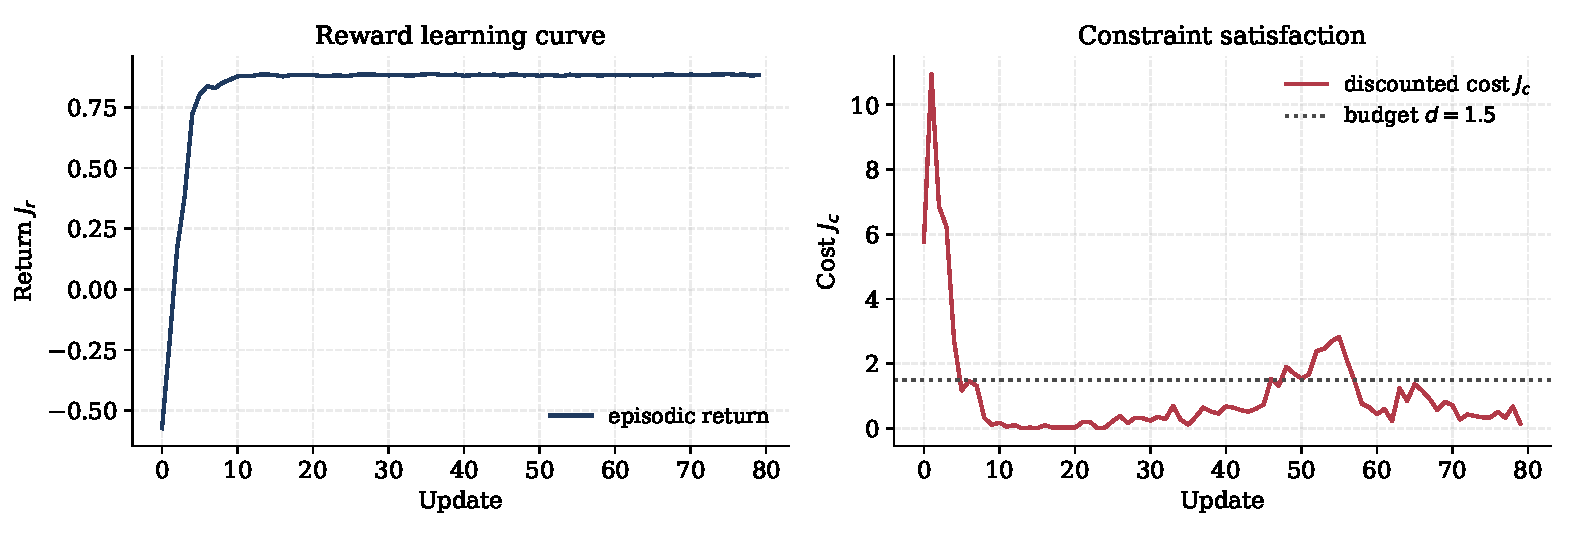
\includegraphics[width=0.95\linewidth]{figs/fig_return_cost.pdf}
  \caption{Left: episodic reward $J_r$. Right: discounted cost $J_c$ tracked
  against the budget $d = 1.5$ (dotted). The policy starts above budget,
  the multiplier spikes, and the agent learns a route that hits the goal
  while skirting lava.}
  \label{fig:return-cost}
\end{figure}

\begin{figure}[h]
  \centering
  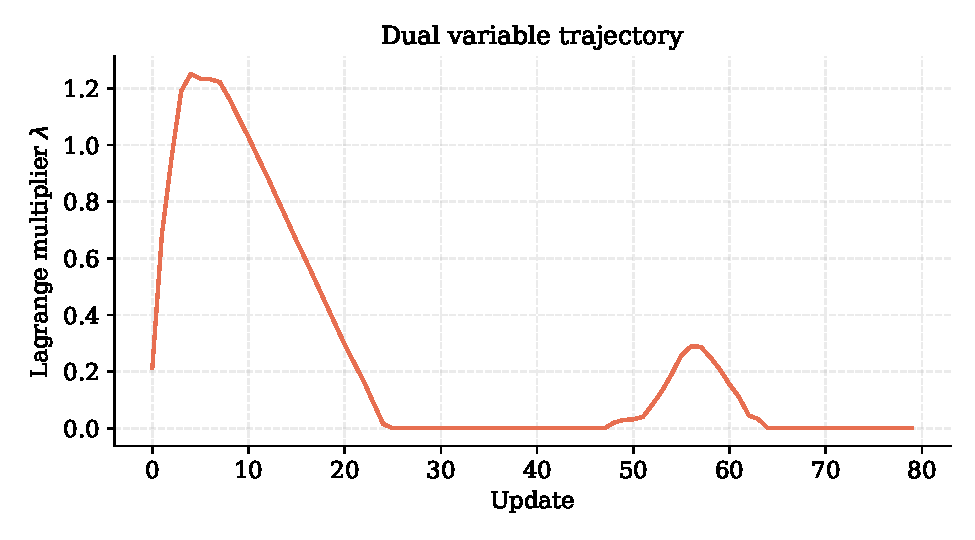
\includegraphics[width=0.7\linewidth]{figs/fig_lambda.pdf}
  \caption{Lagrange multiplier $\lambda$ over training. The sharp early spike
  is the system pricing the constraint violation; it then settles near $0$
  once the agent's cost falls below budget (complementary slackness in
  action).}
  \label{fig:lambda}
\end{figure}

\begin{figure}[h]
  \centering
  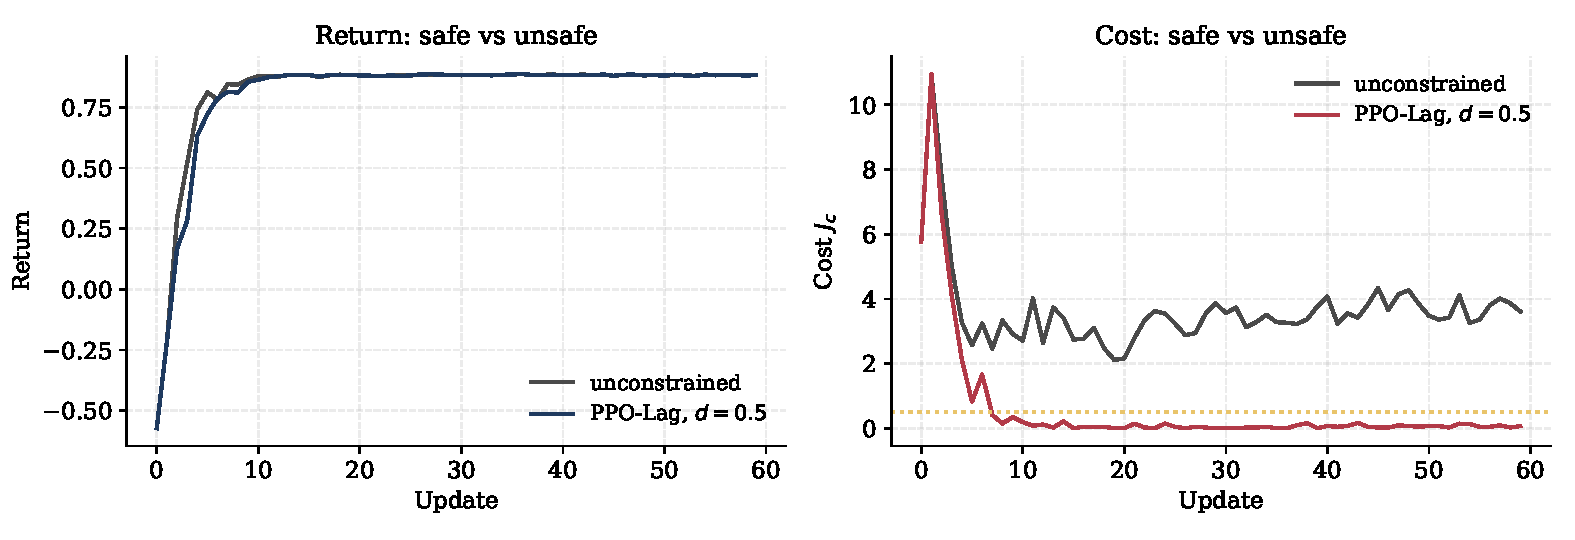
\includegraphics[width=0.95\linewidth]{figs/fig_safe_vs_unsafe.pdf}
  \caption{Strict-budget PPO-Lag ($d=0.5$) vs.\ unconstrained PPO (effectively
  $d = \infty$). The unconstrained policy converges to the shortest path,
  which goes \emph{through} lava and incurs high cost; the constrained
  policy detours, with a small return penalty.}
  \label{fig:safe-vs-unsafe}
\end{figure}

\begin{figure}[h]
  \centering
  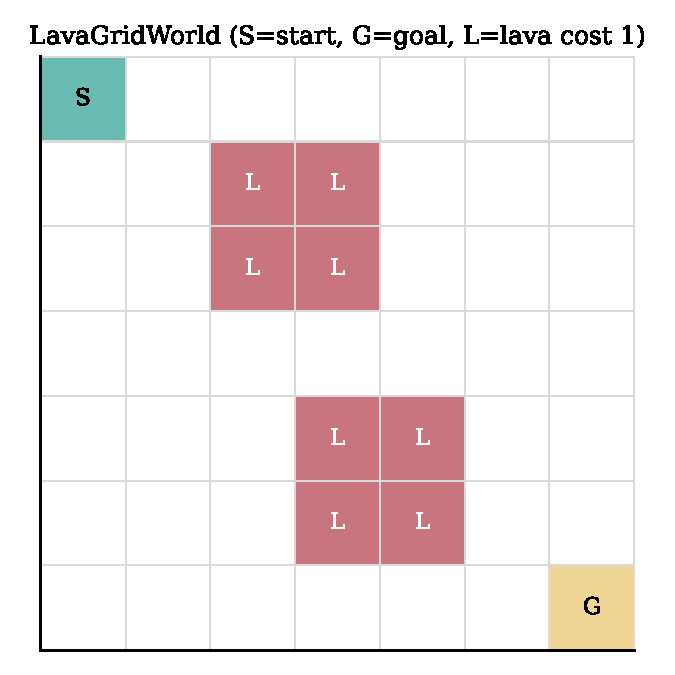
\includegraphics[width=0.4\linewidth]{figs/fig_lavagrid.pdf}
  \caption{The lava gridworld used throughout this chapter.}
  \label{fig:grid}
\end{figure}

\section{Reading the curves}

The cost curve clearly shows the dual mechanism: initial overshoot,
multiplier-driven correction, eventual convergence to a slack value
(below budget). Compare the unconstrained baseline in \cref{fig:safe-vs-unsafe},
which never sees the constraint signal and stays high on cost forever ---
just as the theory predicts.

% =====================================================================
\begin{safetyangle}
The CMDP is the smallest formalism in which ``safety'' is a first-class object
rather than a hyperparameter. But the formalism is not magical:
\begin{itemize}[leftmargin=*]
  \item \textbf{Constraint specification gaming.} The agent only respects the
        constraint you wrote, not the one you meant. If $c$ is ``visits to a
        lava cell'' and the lava also melts the agent, the agent may find a
        policy that minimises lava-visits while never actually completing the
        task --- effectively gaming the constraint. Recommended defence:
        \emph{multiple} cost channels, each capturing one slice of the
        intended safety property (rate, severity, duration).
  \item \textbf{Asymptotic only.} The Lagrangian guarantees feasibility at the
        saddle point. During training there is no guarantee. For real
        deployment you must wrap the policy in a runtime safety filter
        (\emph{week 23}: shielding, CBFs).
  \item \textbf{Multiplier oscillation under cost noise.} The dual update is
        a noisy projected descent on $L$; when $\hat J_c$ has high variance,
        $\lambda$ can oscillate wildly, driving the policy back and forth
        between greedy and risk-averse modes. PID-Lagrangian (Stooke et al.\
        2020, arXiv:2007.03964) damps these oscillations.
\end{itemize}
References: \textsc{Ray, Achiam, Amodei 2019}, arXiv:1910.01708, ``Benchmarking
safe exploration in deep RL''; \textsc{Stooke, Achiam, Abbeel 2020},
arXiv:2007.03964, ``Responsive safety in RL by PID Lagrangian methods''.
\end{safetyangle}

% =====================================================================
\begin{matching}
For the synthetic ATS candidate-matching application, the CMDP form is the
right level of abstraction for fairness. Define:
\begin{itemize}[leftmargin=*]
  \item $r(s,a)$ = match-quality score (skill overlap, recruiter-rating
        proxy) of presenting candidate $a$ in context $s$.
  \item $c(s,a) = \bigl| \,\mathbb{1}[g(a) = \text{minority}] - \rho\,\bigr|$
        where $\rho$ is the target group share and $g(a)$ the candidate's
        protected attribute. A discounted sum of $c$ measures the policy's
        average departure from demographic parity.
  \item $d$ is the maximum tolerated parity gap (set by counsel / DEI policy).
\end{itemize}
PPO-Lagrangian then learns a re-ranking policy that maximises match quality
\emph{subject to} the parity gap not exceeding $d$. The dual variable
$\lambda$ is the marginal cost of one extra unit of parity violation ---
literally what a regulator should be auditing. We will productionise this
exact setup in the week-24 capstone.

For synthetic insurance lead routing the analogue is: $r$ = expected gross-written-premium
contribution; $c$ = saturation of any one broker beyond their capacity quota;
$d$ = broker-quota slack policy. PPO-Lag respects the broker fairness
constraint without manual scalarisation.
\end{matching}

% =====================================================================
\chapter{Exercises}

See \texttt{workbook.ipynb} for graded exercises with hints and an
auto-graded reference. A summary:

\begin{itemize}[leftmargin=*]
  \item \textbf{Ex.\ 1 ($\star$):} one-step Lagrangian dual update.
  \item \textbf{Ex.\ 2 ($\star$):} P3O hinge subgradient.
  \item \textbf{Ex.\ 3 ($\star\star$):} GAE for the cost stream.
  \item \textbf{Ex.\ 4 ($\star\star$):} FOCOPS closed-form non-parametric optimal.
  \item \textbf{Ex.\ 5 ($\star\star$):} empirical CVaR.
  \item \textbf{Ex.\ 6 ($\star\star$):} train PPO-Lag, verify constraint
        satisfaction.
  \item \textbf{Ex.\ 7 ($\star\star\star$):} compare constrained vs.\
        unconstrained; explain the gap.
  \item \textbf{Ex.\ 8 ($\star\star\star$):} PID-Lagrangian one-step update.
\end{itemize}

% =====================================================================
\chapter{Further reading}

The bibliography for this week is in \texttt{extended\_reading.pdf}:
\begin{itemize}[leftmargin=*]
  \item Altman, \emph{Constrained Markov Decision Processes}, CRC 1999 --- the canonical reference.
  \item Ray, Achiam, Amodei, ``Benchmarking safe exploration in deep RL'', arXiv:1910.01708 (2019).
  \item Achiam, Held, Tamar, Abbeel, ``Constrained Policy Optimization'', arXiv:1705.10528 (2017).
  \item Zhang, Vuong, Ross, ``FOCOPS'', arXiv:2002.06506 (2020).
  \item Stooke, Achiam, Abbeel, ``Responsive safety by PID Lagrangian'', arXiv:2007.03964 (2020).
  \item Zhang, Vuong, Ross, ``P3O'', arXiv:2205.11814 (2022).
\end{itemize}

Sourced from \texttt{research/safety\_rl\_sota.md}, sections 1 and 3.

\end{document}
